Мирко "--- большой фанат выкошенных на полях и лугах кругов и других
геометрических объектов предположительно инопланетного происхождения.
Одной летней ночью он решил выкосить свой собственный геометрический
объект на лугу своей бабушки.
Как большой патриот (а также как пациент клиники для душевнобольных),
Мирко решил выкосить объект, который будет иметь форму щитовой части
хорватского герба, которая представляет собой шахматную доску размером
$5 \times 5$ из $13$ красных квадратов и $12$ белых квадратов.


\includegraphics{aliens1.png}


Бабушкин луг представляет собой квадрат, разделённый на $N \times N$
квадратных ячеек одинакового размера.
Ячейка в левом нижнем углу имеет координаты $(1, 1)$, а ячейка в правом
верхнем углу "--- координаты $(N, N)$.
Мирко решил скосить траву только на тех ячейках, которые образуют
на гербе квадраты красного цвета, и оставить остальную траву нескошенной.
Он выбрал нечётное целое число $M \ge 3$ и скосил траву таким образом,
что каждый квадрат шахматной доски соответствует $M \times M$ ячейкам луга,
и шахматная доска целиком располагается внутри луга.

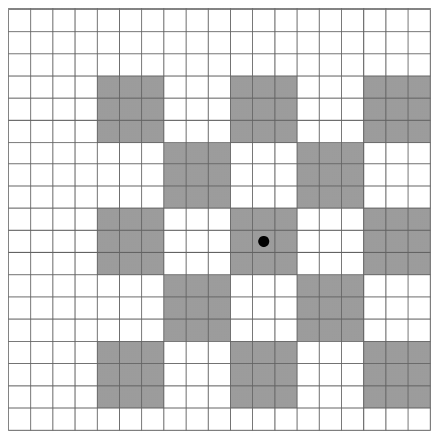
\includegraphics{aliens2.png}

Пример луга и выкошенного Мирко объекта. $N = 19$ и $M = 3$. Ячейки, где трава скошена, показаны серым цветом.	Центр объекта находится в ячейке с координатами $(12, 9)$, отмеченной чёрной точкой.

После того, как Мирко пошел спать, его странное творение привлекло внимание
настоящих инопланетян! 
Летая над лугом в своём космическом корабле, они исследуют с помощью простого
инопланетного устройства объект, выкошенный Мирко.
Это устройство может только определять, скошена трава в некоторой ячейке
или нет.
Инопланетяне обнаружили одну ячейку со скошенной травой и теперь хотят
найти центральную ячейку творения Мирко, чтобы восхититься его красотой.
Однако, они не знают размер квадрата $M$ в объекте, выкошенном Мирко.

Напишите программу, которая по заданному размеру луга $N$ и координатам $(X_0, Y_0)$
одной из ячеек со скошенной травой находит координаты центральной ячейки
выкошенного Мирко объекта посредством общения с инопланетным устройством.
На каждом тесте устройство можно использовать не более $300$ раз.
